\documentclass[aspectratio=169]{beamer}
\setbeamertemplate{navigation symbols}{}
\usepackage{color,amsmath,comment, subfigure}
\usepackage{booktabs}
\def\vf{\vfill}
\usepackage{url}

%\setbeameroption{show notes}

%%%%%%%%%%%%%%%%%%%%%%%%%%
\title[]{Lecture 4: Understanding the small world phenomena}
\author[]{Sociology 204: Social Networks, Spring 2021}
\institute[]{Matthew J. Salganik}
\date[]{
2/2: Small world data and impact

\vfill

\begin{flushleft}
\vspace{0.7in}

\includegraphics[width=0.05\textwidth]{figures/cc.png}
\end{flushleft}
}

\begin{document}
%%%%%%%%%%%%%%%%%%%%%%%%%%%
\frame{\titlepage}

\note{
PREFLIGHT:
ask preceptors to sit in back row

FOR NEXT TIME: This was a bit short and didn't include new stuff, perhaps add some of follow-up work
showing that many things are small world
but not everything: http://www.bbc.com/future/story/20131021-the-medieval-facebook-revealed
}

%%%%%%%%%%%%%%%%%%%%%%%%%%%
\begin{comment}
\begin{frame}

SWBAT:
\begin{enumerate}
\item describe an example where abstract modeling leads to non-intuitive and important insights
\item see an example of similarity of networks across types 
\end{enumerate}

\end{frame}
\end{comment}
%%%%%%%%%%%%%%%%%%%%%%%%
\begin{frame}
\frametitle{}

Are real networks small world networks?

\begin{center}
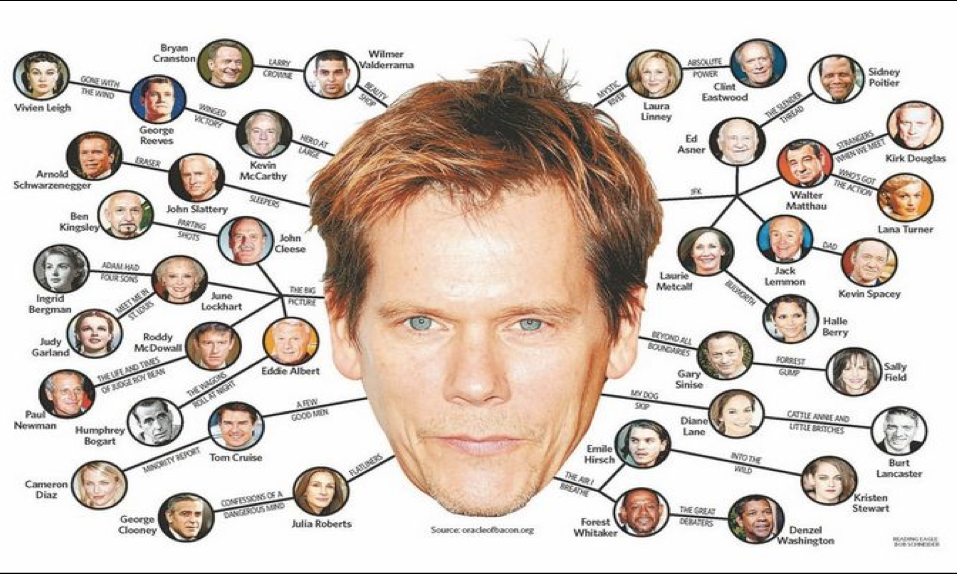
\includegraphics[width = 0.8\textwidth]{figures/degrees_of_bacon}
\end{center}

\end{frame}
%%%%%%%%%%%%%%%%%%%%%%%%%%%%
\begin{frame}
\frametitle{}

Small world means:
\begin{itemize}
\item $L_{actual} \approx L_{random}$
\item $C_{actual} >> C_{random}$
\end{itemize}

\begin{center}
\begin{tabular}{ccccc}
\toprule
 & $L_{actual}$ & $L_{random}$ & $C_{actual}$ & $C_{random}$\\
\midrule
\onslide<2->{Movie actors} & \onslide<3->{3.65} & \onslide<3->{2.99} & \onslide<3->{0.79} & \onslide<3->{0.00027}\\
\onslide<4->{Power Grid} & \onslide<5->{18.7} & \onslide<5->{12.4} & \onslide<5->{0.080} & \onslide<5->{0.005}\\
\onslide<6->{C. Elegans} & \onslide<7->{2.65} & \onslide<7->{2.25} & \onslide<7->{0.28} & \onslide<7->{0.05}\\
\bottomrule
\end{tabular}
\end{center}

\note{Notice that what small world means is slightly different here.  First dataset.  Bam.  Second dataset bam.  Think how excited they are.  Third dataset bam. \\ 
In terms of statistics, there is not statistical significance here.  That's how physicists do statistics.  Extremely simple model suggests a real pattern in three TOTALLY DIFFERENT DATASETS.\\
Since then it has turned up in lots of networks.  This is great science.  When we talked about the Milgram experiment (and Arkadian and the bottlecap factory) who thought that it might apply to worm brains?  Sit down and think about that.\\
}

\end{frame}
%%%%%%%%%%%%%%%%%%%%%%%%%%%
\begin{frame}

Who cares?

\end{frame}
%%%%%%%%%%%%%%%%%%%%%%%%%%%
\begin{frame}
\frametitle{}

\begin{center}
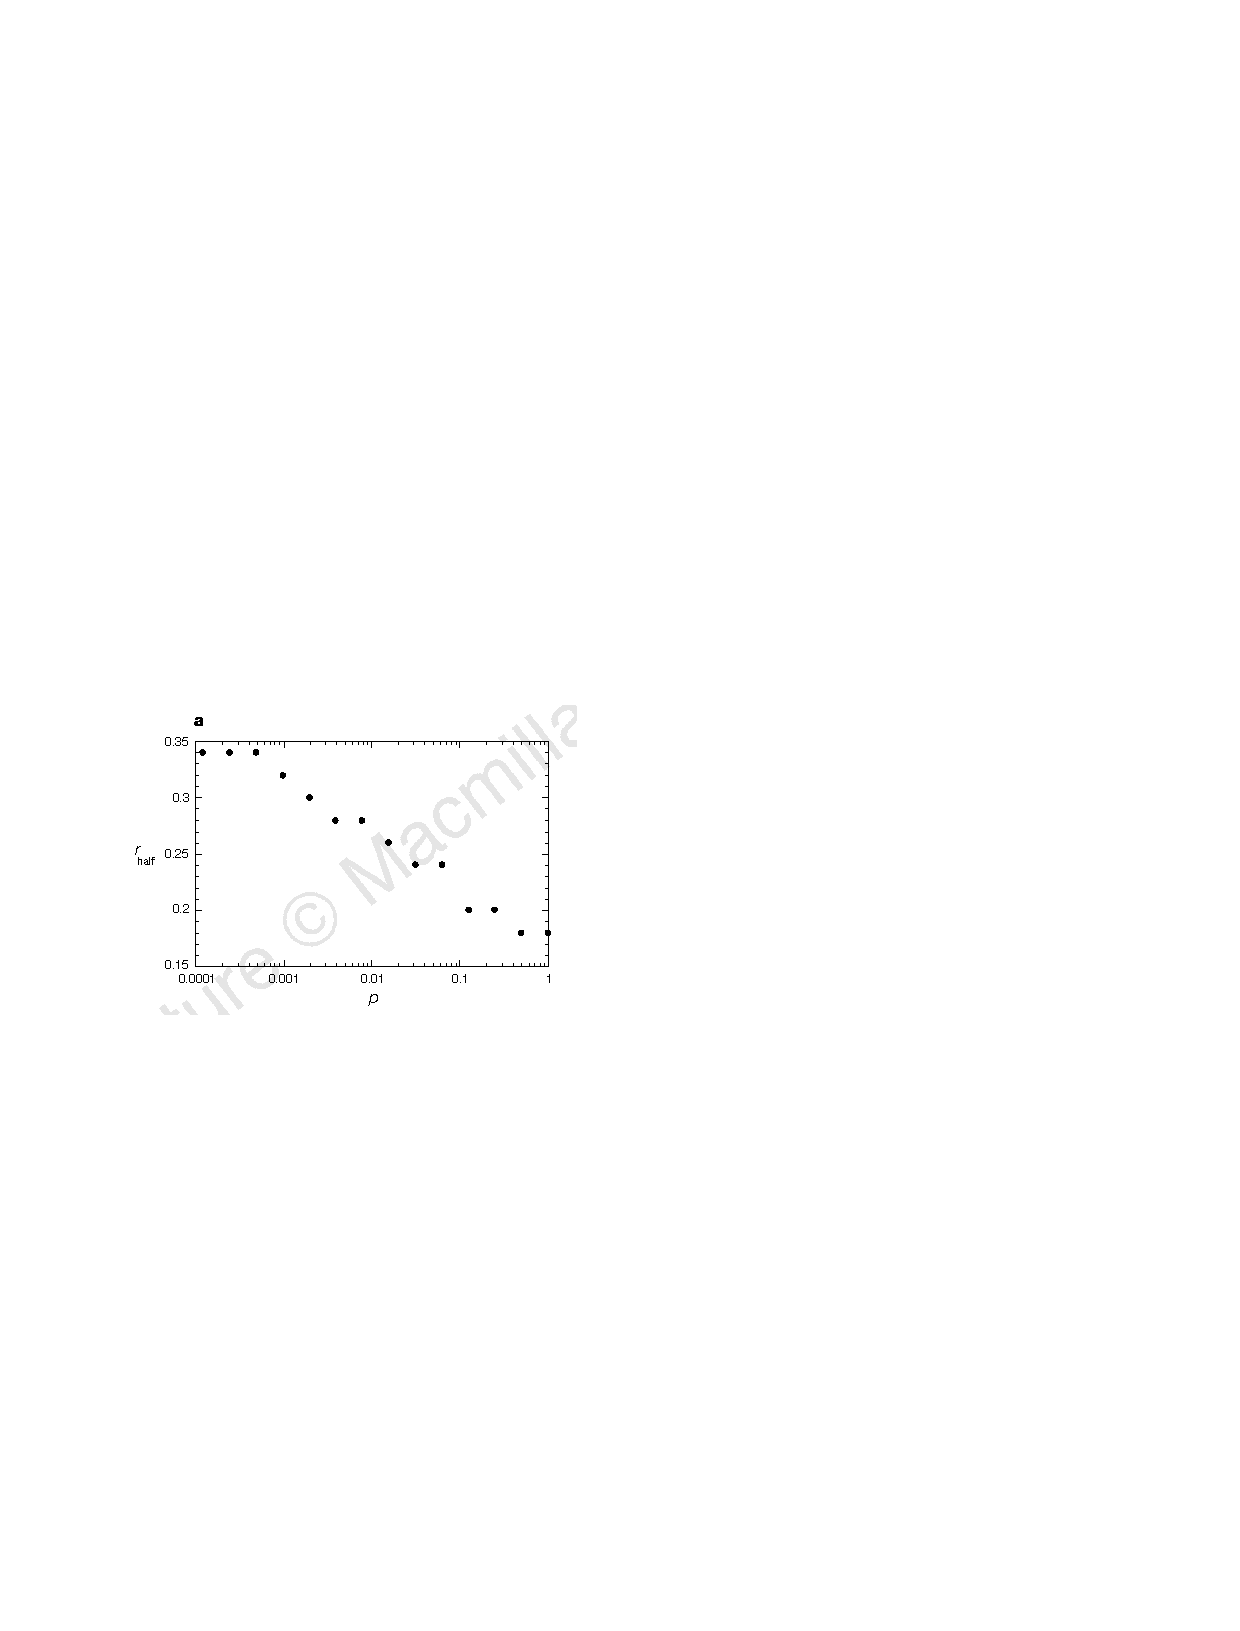
\includegraphics[width = 0.75\textwidth]{figures/watts_collective_1998_fig3a}
\end{center}
\pause

The more shortcuts the less infectious ($r$) a disease needs to be to spread

\note{What is a disease was spreading and $r$ is a measure of the infectiousness of the disease (probability that a neighbor gets infected).  $r_{half}$ is the value of $r$ such that half the population is likely to get infected (let's just say disease takes off).  Small number of shortcuts makes it much easier for a disease to spread (increase in $p$ leads to a decrease in $r_{half}$.}

\end{frame}
%%%%%%%%%%%%%%%%%%%%%%%%%%%
\begin{frame}

\begin{center}
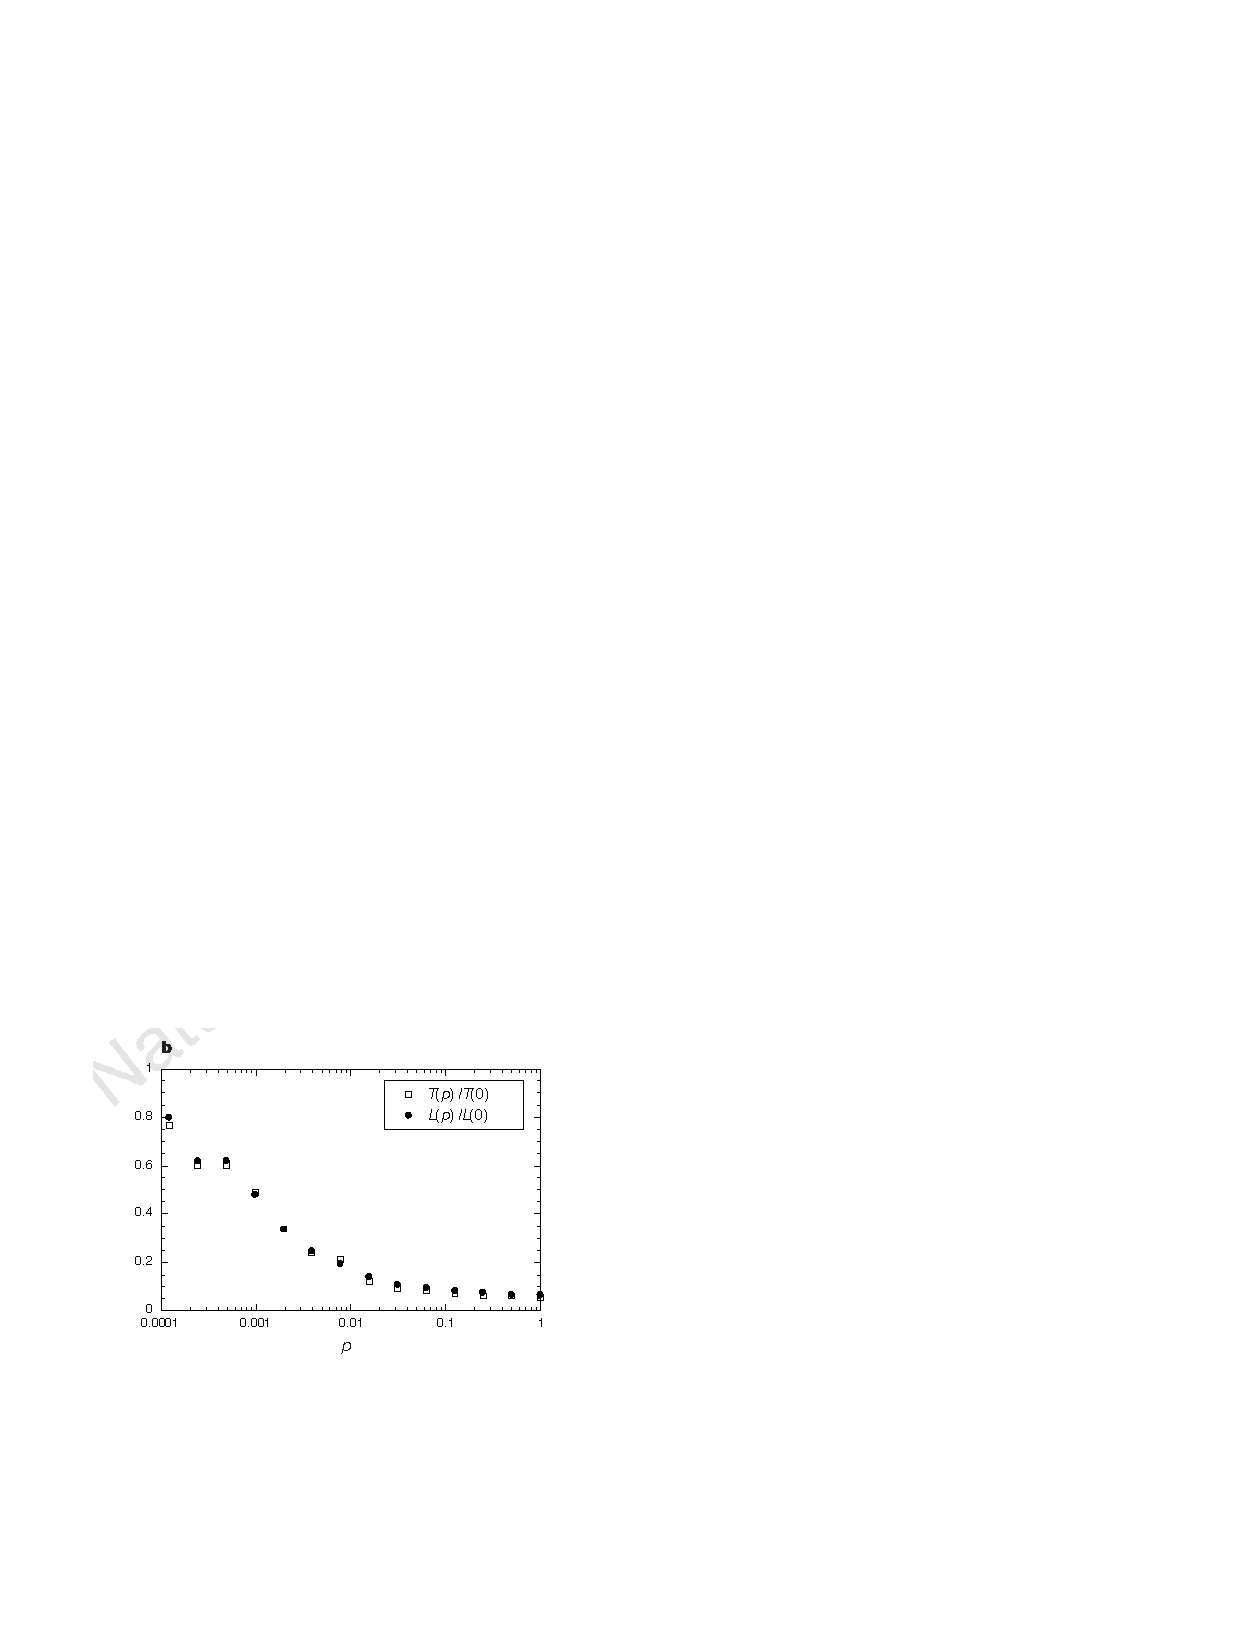
\includegraphics[width = 0.75\textwidth]{figures/watts_collective_1998_fig3b}
\end{center}

\pause

The more shortcuts the faster a disease spreads 

\note{
Time for disease to spread and average path length are basically the same 
}

\end{frame}
%%%%%%%%%%%%%%%%%%%%%%%
\begin{frame}

Making length contractions concrete . . . .

\note{
Sexual network of Princeton students and people in Trenton

A few shortcuts makes everyone close and these shortcuts are completely invisible
}

\end{frame}
%%%%%%%%%%%%%%%%%%%%%%%
\begin{frame}

\begin{itemize}
\item abstract modeling leads to deep and non-obvious insights
\pause
\item shortcuts are key the small world property (characteristic path length changes fast, clustering changes slow)
\pause
\item small local changes can have global impacts
\pause
\item similarity across networks of different types
\pause
\item network structure impacts dynamics 
\end{itemize}

\end{frame}
%%%%%%%%%%%%%%%%%%%%%%%
\begin{frame}

Next class:
\begin{itemize}
\item Watts, Chapter 4, 101-114.
\item Barabasi, A.L. and Bonabeau, E. (2003) Scale-free networks. \textit{Scientific American}, 50-59. (Available from Canvas)
\item Barabasi, A.L. and Albert, R. (1999) The emergence of scaling in random networks. \textit{Science}, 286:509-512.
\item Liljeros, F. et al. (2001). The web of human sexual contacts. \textit{Nature}, 411:907-908 with comment and rejoinder.
\end{itemize}

\note{Another simple model leads to a general network property that turns out to exist in many networks and has impacts for dynamics.}

\end{frame}
%%%%%%%%%%%%%%%%%%%%%%%%%%
\begin{frame}

Please fill out the after lecture feedback survey to me improve the lectures

\end{frame}
%%%%%%%%%%%%%%%%%%%%%%%%%%

\end{document}
